\documentclass[17pt, a2paper, portrait]{tikzposter}

\title{Different Sizes of Infinity}
\author{}
\institute{}

\usepackage{style}

\newcommand{\blu}[1]{{\color{blue}#1}}

\usetheme{Rays}

\begin{document}

\maketitle

\begin{columns}
\column{1.0}
\block{Preamble}
{
In Toy Story, Buzz Lightyear's famous catchphrase is ``\textbf{To Infinity and Beyond!}''. But what does \emph{beyond infinity} mean? Is there anything larger than infinity?

In this poster, we will explore the different ``sizes'' of infinity, where one infinity can indeed be ``larger'' than another.

We shall assume familiarity with logic notation and set notation. Remember that infinity is a concept, \emph{not} a number.
}

%\column{0.3}
%\block{~}
%{
%\begin{figure}[H]
%    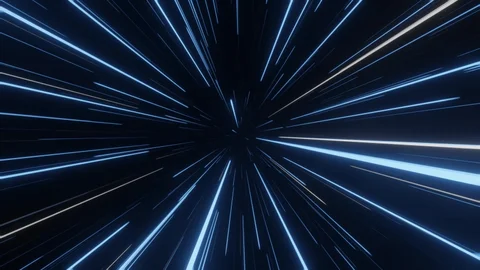
\includegraphics[width=0.25\textwidth]{images/infinity.png}
%\end{figure}
%}
\end{columns}

\begin{columns}
\column{0.5}
\block{Functions}
{
%A \vocab{set}, defined loosely, is simply a collection of \vocab{elements}.

A \vocab{function} $f:X\to Y$ is a mapping of \emph{every} element of $X$ to exactly one element of $Y$; we call $X$ and $Y$ the \vocab{domain} and \vocab{codomain} of $f$ respectively.

$f:X\to Y$ is \vocab{injective} (or \emph{one-to-one}) if each element of $Y$ has at most one element of $X$ that maps to it.
\[ \forall x_1,x_2\in X,\:f(x_1)=f(x_2) \implies x_1=x_2 \]

$f:X\to Y$ is \vocab{surjective} (or \emph{onto}) if \emph{every} element of $Y$ is mapped to at least one element of $X$.
\[ \forall y\in Y,\:\exists x\in X \suchthat f(x)=y \]

$f:X\to Y$ is \vocab{bijective} (one-to-one correspondence) if it is both injective and surjective: each element of $Y$ is mapped to a unique element of $X$.

%\begin{figure}[H]
%    \hspace*{0cm}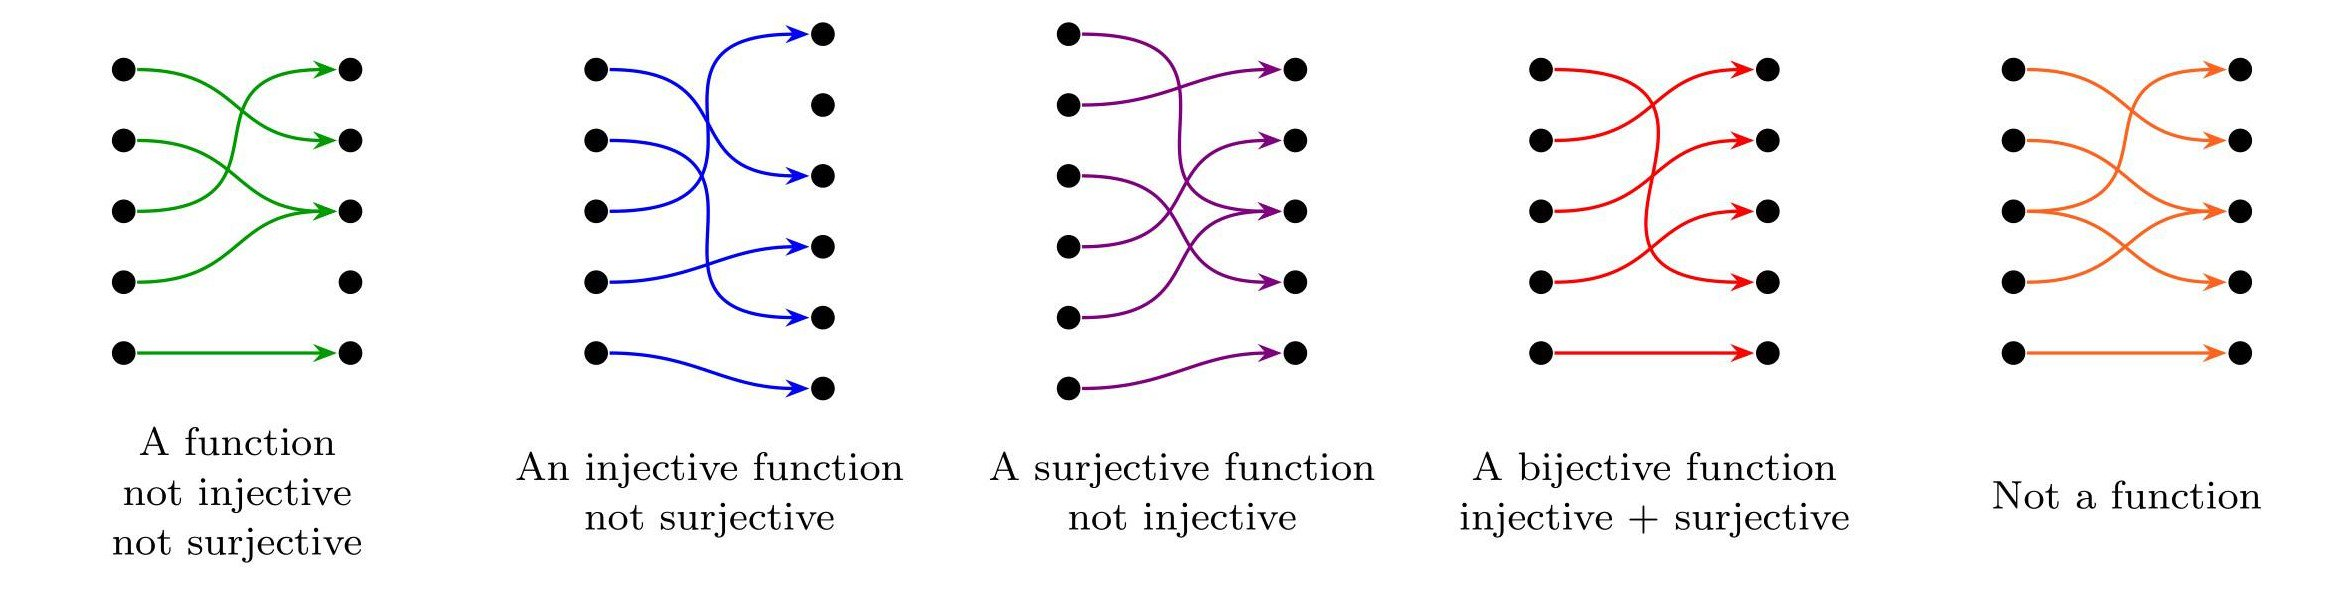
\includegraphics[width=0.4\textwidth]{images/functions.jpeg}
%\end{figure}
}

\column{0.5}
\block{Cardinality and countable sets}
{
$X$ and $Y$ have the same \vocab{cardinality}, denoted by $|X|=|Y|$, if there exists a bijection $f:X\to Y$, i.e. two sets have the same size when you can pair each element in one set with a unique element in the other.

The empty set $\emptyset$ is finite and has cardinality $|\emptyset|\coloneqq0$; a non-empty set $X$ is said to be \vocab{finite} and have cardinality $|X|=n\in\ZZ^+$ if and only if there exists a bijection from $X$ to the set $\{1,2,\dots,n\}$.

Generalising this notion, a set $X$ is \vocab{countably infinite} if it has the same cardinality as the set $\ZZ^{+}$. (This means that to show that $X$ is countably infinite, we need to show that there is a bijection between it and $\ZZ^+$.)

A set $X$ is \vocab{countable} if it is either \emph{finite}, or \emph{countably infinite}; $X$ is \vocab{uncountable} if it is not countable.
}
\end{columns}

\begin{columns}
\column{0.5}
\block{$2\ZZ^+$, $\ZZ$}
{
\textbf{\textsf{Is the set of positive even integers larger or smaller than the set of positive integers?}}

\textbf{Answer:} $|2\ZZ^+|=|\ZZ^+|$ as $2\ZZ^+$ is countably infinite.

%\begin{wrapfigure}{r}{0.15\textwidth}
%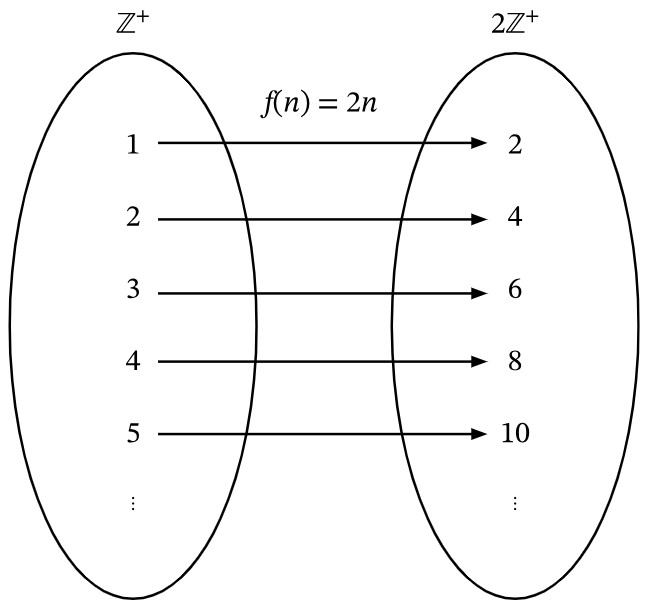
\includegraphics[width=\linewidth]{images/Z+_2Z+.jpg} 
%\end{wrapfigure}

Since there exists a bijection $f:\ZZ^+\to2\ZZ^+$ given by $f(n)=2n$, hence $2\ZZ^+$ is countably infinite.

\

\textbf{\textsf{Is the set of integers larger or smaller than the set of positive integers?}}

\textbf{Answer:} $|\ZZ|=|\ZZ^+|$ as $\ZZ$ is countably infinite.

%\begin{wrapfigure}{r}{0.20\textwidth}
%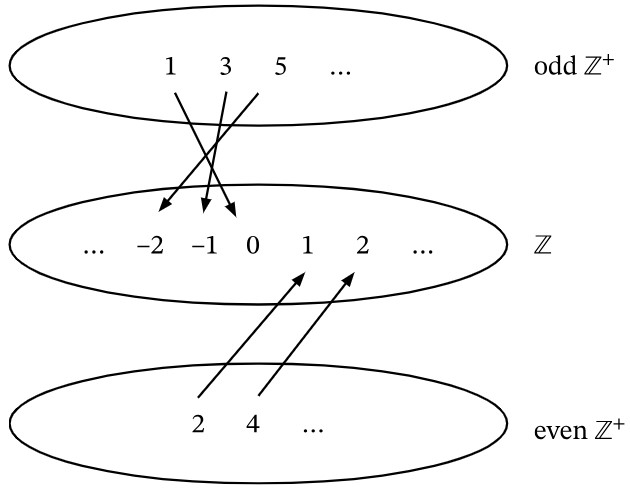
\includegraphics[width=\linewidth]{images/Z+_Z.jpg} 
%\end{wrapfigure}

Since there exists a bijection $f:\ZZ^+\to\ZZ$ given by
\[ f(n)=\begin{cases}
\begin{aligned}
\frac{n}{2} \quad & \text{ if } n \text{ is even} \\[1ex]
\frac{1-n}{2} & \text{ if } n \text{ is odd}
\end{aligned}
\end{cases} \]
where $f(1)=0$, $f(2)=1$, $f(3)=-1$, $f(4)=2$, $f(5)=-2$, $f(6)=3,\dots$, i.e. our function $f$ stretches in both positive and negative directions to cover both positive and negative integers, hence $\ZZ$ is countably infinite.
}
%\begin{flushright}
%\textbf{Created by Ryan Joo Rui An}
%\end{flushright}

\column{0.5}
\block{$\RR$}
{
\textbf{\textsf{Is the set of real numbers larger or smaller than the set of positive integers?}}

\textbf{Answer:} $|\RR|>|\ZZ^+|$ as $\RR$ is uncountable.

To prove that $\RR$ is uncountable, we show that the interval $(0,1)$ is uncountable, which implies the uncountability of $\RR$ as $(0,1)$ is a subset of $\RR$. Assume otherwise, that $(0,1)$ is countable and there exists a bijection $f:\ZZ^+\to(0,1)$:
\begin{align*}
f(1) &= 0.\blu{a_{1,1}}\:a_{1,2}\:a_{1,3}\:a_{1,4}\:a_{1,5}\:\cdots \\
f(2) &= 0.a_{2,1}\:\blu{a_{2,2}}\:a_{2,3}\:a_{2,4}\:a_{2,5}\:\cdots
%f(3) &= 0.a_{3,1}\:a_{3,2}\:\blu{a_{3,3}}\:a_{3,4}\:a_{3,5}\:\cdots 
%f(4) &= 0.a_{4,1}\:a_{4,2}\:a_{4,3}\:\blu{a_{4,4}}\:a_{4,5}\:\cdots \\
%f(5) &= 0.a_{5,1}\:a_{5,2}\:a_{5,3}\:a_{5,4}\:\blu{a_{5,5}}\:\cdots
\end{align*}
\[ \vdots \]
where $f(i)$ denotes the $i$-th real number, and each $a_{i,j}$ is some arbitrary non-negative integer.

Define a new real number $b=0.b_1\:b_2\:b_3\:b_4\:b_5\:\cdots$, where $b_i \neq a_{i,i}$ for all $i\in\ZZ^+$. $b$ differs from every $f(i)$ at least at the $i$-th decimal place. Hence $b$ is not in our above list, implying $f$ is not surjective and thus not bijective. Thus $(0,1)$ is uncountable, and consequently, $\RR$ is uncountable.
}
\end{columns}

\end{document}